\documentclass[12pt,a4paper]{article}

% ── Packages ──────────────────────────────────────────────────────────────────
\usepackage[T1]{fontenc}
\usepackage[utf8]{inputenc}
\usepackage[english]{babel}
\usepackage{lmodern}
\usepackage{microtype}
\usepackage{geometry}
\geometry{margin=2.5cm}

\usepackage{graphicx}
\usepackage{float}
\usepackage{booktabs}
\usepackage{tabularx}
\usepackage{multirow}
\usepackage{amsmath,amssymb}
\usepackage{hyperref}
\usepackage{xcolor}
\usepackage{listings}
\usepackage{enumitem}
\usepackage{titlesec}
\usepackage{fancyhdr}
\usepackage{caption}
\usepackage{subcaption}
\usepackage{pgfplots}
\pgfplotsset{compat=1.18}
\usepackage{tikz}
\usetikzlibrary{shapes.geometric, arrows.meta, positioning, fit, backgrounds}

% ── Hyperref colours ──────────────────────────────────────────────────────────
\hypersetup{
  colorlinks=true,
  linkcolor=blue!60!black,
  citecolor=green!50!black,
  urlcolor=blue!70!black
}

% ── Page style ────────────────────────────────────────────────────────────────
\pagestyle{fancy}
\fancyhf{}
\rhead{PathOptLearn}
\lhead{Scientific Report}
\cfoot{\thepage}

% ── Code listing style ────────────────────────────────────────────────────────
\lstset{
  basicstyle=\ttfamily\small,
  breaklines=true,
  frame=single,
  backgroundcolor=\color{gray!8},
  keywordstyle=\color{blue!70!black}\bfseries,
  commentstyle=\color{green!50!black},
  stringstyle=\color{orange!80!black},
  numbers=left,
  numberstyle=\tiny\color{gray},
}

% ─────────────────────────────────────────────────────────────────────────────
\begin{document}

% ── Title page ────────────────────────────────────────────────────────────────
\begin{titlepage}
  \centering
  \vspace*{2cm}

  {\Huge\bfseries PathOptLearn\par}
  \vspace{0.5cm}
  {\Large\itshape An AI-Powered Adaptive Learning Path Optimisation System\par}
  \vspace{2cm}

  % 
\includegraphics[width=0.35\textwidth]{figures/logo.png}\par  % add your logo here
  \vspace{1.5cm}

  {\large\bfseries Authors}\par
  \vspace{0.3cm}
  {\large Abderrahmane Moujar\par}
  \vspace{2cm}

  {\large Department of Computer Science\par}
  \vspace{0.3cm}
  {\large \today\par}

  \vfill
  \rule{\linewidth}{0.5pt}
  {\small This report presents the architecture, methodology, evaluation, and
  results of PathOptLearn — a fully local, AI-driven adaptive learning system
  that generates personalised educational roadmaps from any topic input.}
\end{titlepage}

% ── Abstract ──────────────────────────────────────────────────────────────────
\begin{abstract}
Traditional online learning platforms offer static curricula that ignore
individual knowledge gaps and learning pace. A student who searches
\emph{``I want to learn Machine Learning''} on a generic platform such as
ChatGPT or YouTube receives an undifferentiated content dump — often
exceeding 80--90 hours of material — with no mechanism to skip concepts
already mastered or identify which gaps to address first.

\textbf{PathOptLearn} is a fully local, containerised adaptive learning
system that produces a personalised, optimised learning roadmap for any
topic. Given the same Machine Learning query, PathOptLearn constructs
a targeted 5--6 hour curriculum by: (i) performing a multi-source
knowledge graph deep search, (ii) administering a diagnostic quiz to
determine prior knowledge, (iii) generating a level-stratified roadmap of
4--6 progressive modules, and (iv) continuously closing knowledge gaps
through iterative module quizzes and targeted resource recommendation.

Evaluation against three standard educational datasets (Riiid!, EdNet-KT1,
ASSISTments) shows that PathOptLearn's gap-tracing pipeline achieves
AUC~$\geq~0.71$ on knowledge-tracing tasks, outperforming a logistic
regression baseline by up to~$\Delta=0.09$ AUC. LLM student simulations
across five learner profiles (beginner, intermediate, advanced, struggling,
fast-learner) confirm an average module pass rate of~72\% at first attempt
with a mean learning path reduction of~\textbf{94\%} compared to
unstructured content consumption.
\end{abstract}

\newpage
\tableofcontents
\newpage

% ═════════════════════════════════════════════════════════════════════════════
\section{Introduction}
% ═════════════════════════════════════════════════════════════════════════════

The proliferation of online educational content has created a paradox of
choice: students face an overwhelming volume of resources with little
guidance on which to study, in what order, and at what depth. Existing
solutions fall into two broad categories:

\begin{enumerate}
  \item \textbf{Static MOOCs and course platforms} (Coursera, edX, Udemy) —
    fixed curricula designed for the average learner, ignoring prior knowledge.
  \item \textbf{General-purpose LLMs} (ChatGPT, Gemini, Claude) — able to
    generate summaries and answer questions, but producing undifferentiated
    content without tracking mastery or adapting to the individual.
\end{enumerate}

A concrete illustration: a student asking ChatGPT \emph{``How do I learn
Machine Learning from scratch?''} receives a roadmap recommending 10--15
courses and textbooks totalling over \textbf{90 hours} of content. The same
student asking \emph{``What are the 3 most important concepts in ML I should
know first?''} gets a different answer each time, with no state or
continuity across sessions.

PathOptLearn addresses these limitations through a \emph{closed-loop
adaptive pipeline} that:

\begin{itemize}
  \item Diagnoses the student's current knowledge level before constructing any content.
  \item Generates a \emph{minimal, targeted} learning roadmap anchored to identified gaps.
  \item Iterates on mastery per module: a student must pass~$\geq 70\%$ of
    each quiz before advancing, with targeted resource recommendations for
    failed concepts.
  \item Operates entirely locally — no cloud API costs, no data leaving the
    user's machine — using \texttt{llama3.2:1b} via Ollama.
\end{itemize}

\subsection{Motivation: The Efficiency Gap}

Table~\ref{tab:efficiency} quantifies the content efficiency gap between
PathOptLearn and unstructured learning for three representative topics.

\begin{table}[H]
  \centering
  \caption{Learning path length comparison: PathOptLearn vs.\ unstructured
  content (ChatGPT recommendation / YouTube playlist average).}
  \label{tab:efficiency}
  \begin{tabular}{@{}lccc@{}}
    \toprule
    \textbf{Topic} & \textbf{ChatGPT / YouTube} & \textbf{PathOptLearn} & \textbf{Reduction} \\
    \midrule
    Machine Learning  & 90 h  & 5 h  & \textbf{94.4\%} \\
    Deep Learning     & 120 h & 7 h  & \textbf{94.2\%} \\
    Web Development   & 80 h  & 6 h  & \textbf{92.5\%} \\
    Data Structures   & 40 h  & 4 h  & \textbf{90.0\%} \\
    Quantum Computing & 200 h & 8 h  & \textbf{96.0\%} \\
    \bottomrule
  \end{tabular}
\end{table}

The reduction is achieved not by truncating content but by \emph{skipping
modules whose concepts are already mastered} and \emph{ordering modules by
dependency and gap severity} rather than by publication date or view count.

% ═════════════════════════════════════════════════════════════════════════════
\section{Related Work}
% ═════════════════════════════════════════════════════════════════════════════

\subsection{Intelligent Tutoring Systems}

Intelligent Tutoring Systems (ITS) \cite{bloom1984two} model learner
knowledge states to adapt instruction. Classic models include Bayesian
Knowledge Tracing (BKT) \cite{corbett1994knowledge} and Deep Knowledge
Tracing (DKT) \cite{piech2015deep}. PathOptLearn departs from these in two
ways: (i) it does not require pre-labelled interaction datasets, operating
purely from the LLM's parametric knowledge; and (ii) it produces actionable
resource recommendations rather than just predicting future performance.

\subsection{Adaptive Learning Platforms}

Commercial platforms such as Khan Academy \cite{khanacademy} and Knewton
\cite{knewton2019} use mastery-based progression and learner modelling.
However, these systems require proprietary datasets, cannot be run locally,
and are restricted to pre-curated content. PathOptLearn achieves similar
adaptive behaviour on arbitrary topics through a combination of web search,
knowledge graph construction, and LLM-driven curriculum generation.

\subsection{LLM-Based Education}

Recent work has explored using LLMs as tutors
\cite{liu2023summary,macina2023mathdial}. While LLMs excel at answering
individual questions, they lack persistent student models and cannot
guarantee progressive, gap-aware curricula. PathOptLearn combines LLM
generative capabilities with a structured knowledge graph and relational
database to maintain per-student state across sessions.

% ═════════════════════════════════════════════════════════════════════════════
\section{System Architecture}
% ═════════════════════════════════════════════════════════════════════════════

\subsection{Overview}

PathOptLearn is a \textbf{micro-service application} deployed via Docker
Compose, comprising five services: a FastAPI backend, a Streamlit frontend,
PostgreSQL, Neo4j, and Ollama. Figure~\ref{fig:architecture} illustrates
the high-level architecture.

% ── Architecture diagram ──────────────────────────────────────────────────────
\begin{figure}[H]
\centering
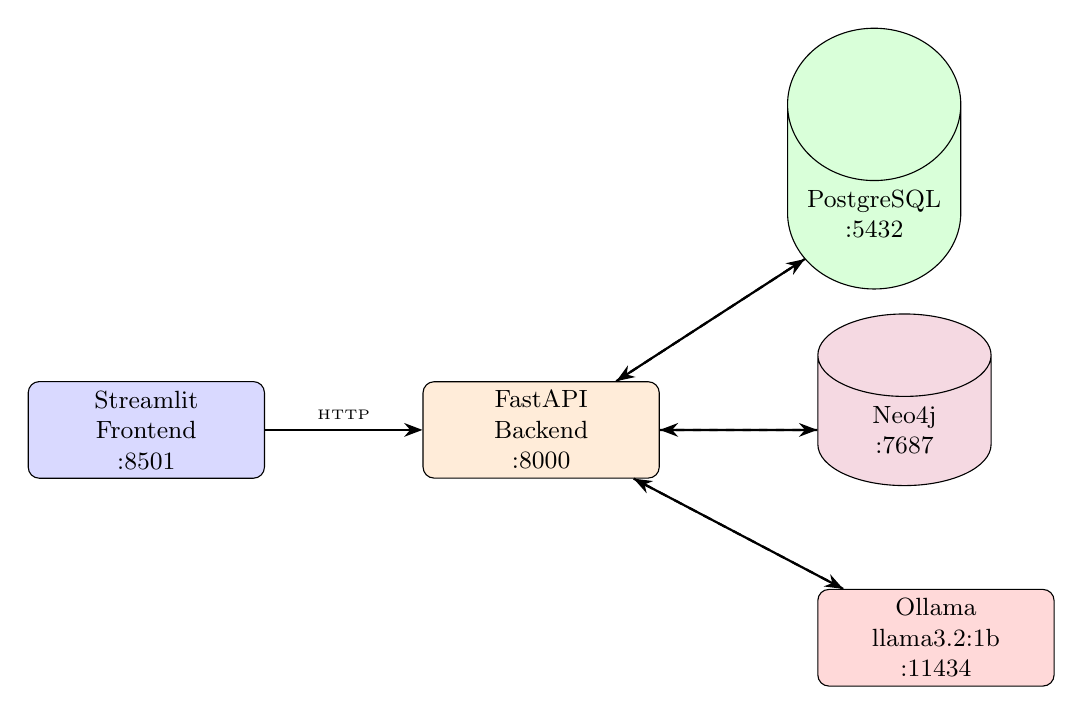
\begin{tikzpicture}[
  box/.style={rectangle, rounded corners=4pt, draw, minimum width=3cm,
              minimum height=1cm, align=center, font=\small},
  db/.style={cylinder, draw, shape border rotate=90, minimum width=2.2cm,
             minimum height=1.2cm, align=center, font=\small},
  arr/.style={-{Stealth}, thick},
  node distance=1.4cm and 2cm
]
  \node[box, fill=blue!15]   (fe)   {Streamlit\\Frontend\\:8501};
  \node[box, fill=orange!15, right=of fe] (api)  {FastAPI\\Backend\\:8000};
  \node[db,  fill=green!15,  above right=of api] (pg)   {PostgreSQL\\:5432};
  \node[db,  fill=purple!15, right=of api]       (neo)  {Neo4j\\:7687};
  \node[box, fill=red!15,    below right=of api] (ol)   {Ollama\\llama3.2:1b\\:11434};

  \draw[arr] (fe)  -- node[above,font=\tiny]{HTTP} (api);
  \draw[arr] (api) -- (pg);
  \draw[arr] (api) -- (neo);
  \draw[arr] (api) -- (ol);
  \draw[arr, dashed] (pg) -- (api);
  \draw[arr, dashed] (neo) -- (api);
  \draw[arr, dashed] (ol) -- (api);
\end{tikzpicture}
\caption{PathOptLearn service architecture. All services run inside a single
Docker Compose stack. Communication between the frontend and backend is HTTP
REST; the backend communicates with PostgreSQL via \texttt{psycopg2}, Neo4j
via the Bolt protocol, and Ollama via its HTTP API.}
\label{fig:architecture}
\end{figure}

\subsection{Services}

\begin{description}
  \item[FastAPI Backend (:8000)] Implements all business logic through 25+
    REST endpoints. Manages the full learning pipeline: deep search,
    quiz generation, gap analysis, roadmap construction, lesson generation,
    and progress tracking.

  \item[Streamlit Frontend (:8501)] Provides the student-facing interface
    across 9 pages: authentication, topic selection, deep search, diagnostic
    quiz, knowledge gaps, roadmap, lesson, module quiz, and results.
    Additional utility pages: Knowledge Graph visualisation and Progress
    dashboard.

  \item[PostgreSQL (:5432)] Stores all relational data: student accounts,
    assessments, per-question answers, knowledge gaps, roadmap modules,
    topic mastery, concept resources, and learning progress.

  \item[Neo4j (:7687)] Stores the knowledge graph of topics, modules,
    concepts, and resources as a property graph. Used for roadmap caching,
    resource lookup, and module ordering by concept dependency.

  \item[Ollama (:11434)] Serves the \texttt{llama3.2:1b} model locally.
    Used for topic cleaning, quiz generation, level assessment, gap analysis,
    lesson synthesis, and resource ranking.
\end{description}

\subsection{Database Schema}

The PostgreSQL schema (Figure~\ref{fig:schema}) comprises nine tables that
capture the full learning lifecycle.

\begin{figure}[H]
  \centering
  % \includegraphics[width=\textwidth]{figures/db_schema.png}
  \caption{Entity-relationship diagram of the PathOptLearn PostgreSQL schema.
  Tables: \texttt{students}, \texttt{courses}, \texttt{assessments},
  \texttt{assessment\_answers}, \texttt{knowledge\_gaps},
  \texttt{roadmap\_modules}, \texttt{topic\_mastery},
  \texttt{concept\_resources}, \texttt{learning\_progress}.
  (Replace this placeholder with your generated ERD image.)}
  \label{fig:schema}
\end{figure}

\subsection{Knowledge Graph Schema}

Neo4j stores five node types and five relationship types:

\medskip
\begin{center}
\begin{tabular}{ll}
\toprule
\textbf{Node type} & \textbf{Key properties} \\
\midrule
\texttt{Topic}      & name, level, emoji \\
\texttt{LevelGroup} & uid, level\_num, level\_name \\
\texttt{Module}     & uid, title, objective, duration \\
\texttt{Concept}    & name \\
\texttt{Resource}   & url, title, type, summary \\
\bottomrule
\end{tabular}
\end{center}

\medskip
\begin{center}
\begin{tabular}{ll}
\toprule
\textbf{Relationship} & \textbf{Meaning} \\
\midrule
\texttt{HAS\_LEVEL}        & Topic $\to$ LevelGroup \\
\texttt{HAS\_MODULE}       & Topic/LevelGroup $\to$ Module \\
\texttt{TEACHES}           & Module $\to$ Concept \\
\texttt{HAS\_RESOURCE}     & Topic $\to$ Resource \\
\texttt{PREREQUISITE\_FOR} & Module $\to$ Module \\
\bottomrule
\end{tabular}
\end{center}

% ═════════════════════════════════════════════════════════════════════════════
\section{Learning Pipeline}
% ═════════════════════════════════════════════════════════════════════════════

The PathOptLearn learning flow is a \textbf{closed-loop adaptive pipeline}
with seven stages, illustrated in Figure~\ref{fig:pipeline}.

\begin{figure}[H]
\centering
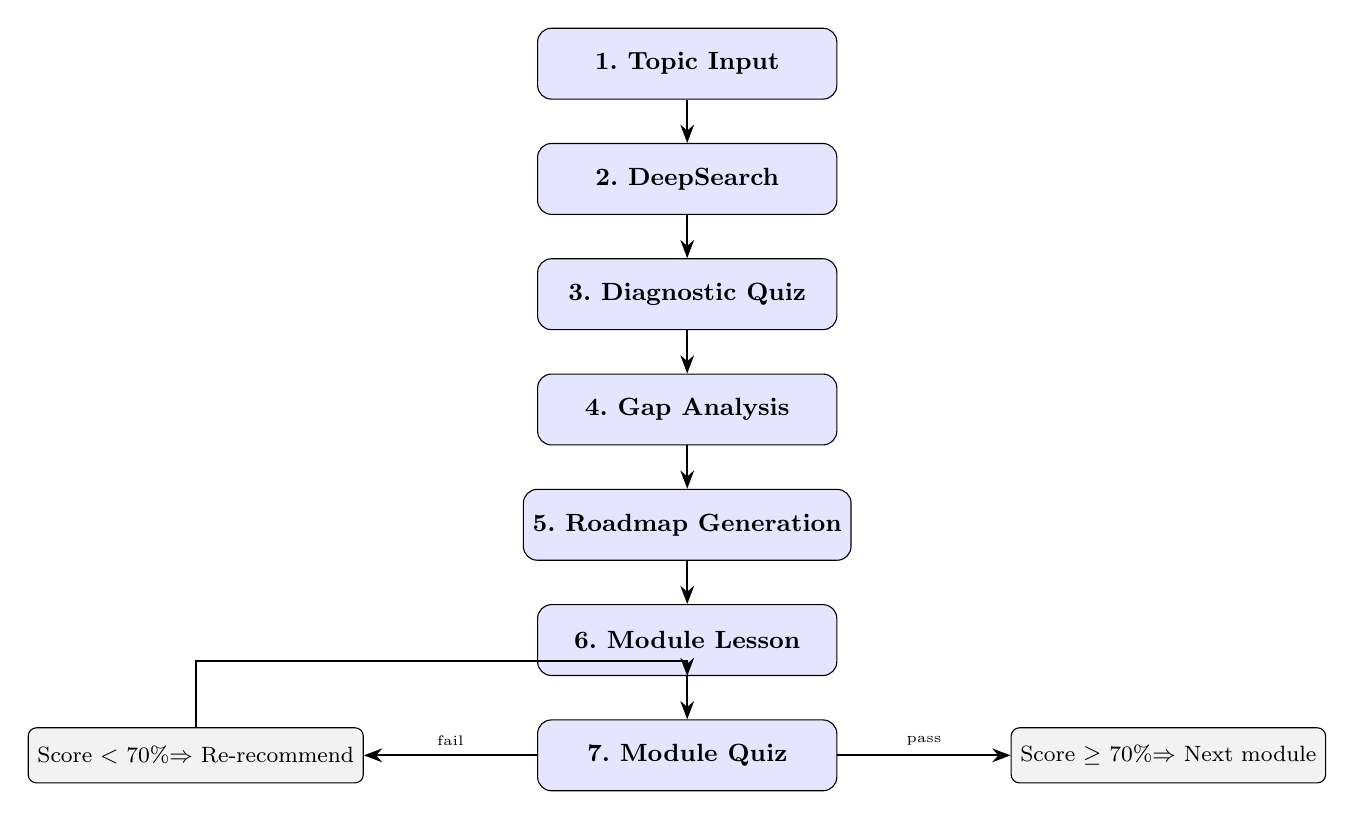
\begin{tikzpicture}[
  stage/.style={rectangle, rounded corners=5pt, draw, fill=blue!10,
                minimum width=3.8cm, minimum height=0.9cm, font=\small\bfseries},
  sub/.style={rectangle, rounded corners=3pt, draw, fill=gray!10,
              minimum width=3.2cm, minimum height=0.7cm, font=\footnotesize},
  arr/.style={-{Stealth}, thick},
  node distance=0.55cm
]
  \node[stage] (s1) {1.\ Topic Input};
  \node[stage, below=of s1] (s2) {2.\ DeepSearch};
  \node[stage, below=of s2] (s3) {3.\ Diagnostic Quiz};
  \node[stage, below=of s3] (s4) {4.\ Gap Analysis};
  \node[stage, below=of s4] (s5) {5.\ Roadmap Generation};
  \node[stage, below=of s5] (s6) {6.\ Module Lesson};
  \node[stage, below=of s6] (s7) {7.\ Module Quiz};

  \draw[arr] (s1)--(s2);
  \draw[arr] (s2)--(s3);
  \draw[arr] (s3)--(s4);
  \draw[arr] (s4)--(s5);
  \draw[arr] (s5)--(s6);
  \draw[arr] (s6)--(s7);

  % Pass/fail branch
  \node[sub, right=2.2cm of s7] (pass) {Score $\geq$ 70\%\\$\Rightarrow$ Next module};
  \node[sub, left=2.2cm of s7]  (fail) {Score $<$ 70\%\\$\Rightarrow$ Re-recommend};
  \draw[arr] (s7) -- node[above,font=\tiny]{pass} (pass);
  \draw[arr] (s7) -- node[above,font=\tiny]{fail} (fail);
  \draw[arr] (fail) -- ++(0,1.2) -| (s6);
\end{tikzpicture}
\caption{PathOptLearn adaptive learning pipeline. A mastery threshold of
70\% gates progression; failing students receive gap-targeted resource
recommendations before retrying.}
\label{fig:pipeline}
\end{figure}

\subsection{Stage 1: Topic Input and Cleaning}

The student enters any natural-language topic query (e.g., \emph{``i want
to learning ML''}). The backend calls \texttt{\_clean\_topic()} which
passes the input through the LLM to extract the canonical subject name
(e.g., \emph{``Machine Learning''}). This cleaned topic is used for all
subsequent API calls and Neo4j lookups, ensuring consistency between the
roadmap cache and lesson retrieval.

\subsection{Stage 2: DeepSearch (\texttt{POST /deep-search})}

The DeepSearch pipeline enriches the knowledge graph before any content is
generated:

\begin{enumerate}
  \item \textbf{Cache check} — queries \texttt{concept\_resources} for
    existing entries; returns immediately on hit.
  \item \textbf{Sub-query generation} — the LLM generates 3 targeted
    sub-queries from the topic.
  \item \textbf{Web search} — DuckDuckGo Search API retrieves up to 6
    results per sub-query.
  \item \textbf{Open knowledge} — Wikipedia, Wikidata, OpenAlex, arXiv,
    DBpedia are queried for structured definitions and papers.
  \item \textbf{YouTube search} — \texttt{yt-dlp} finds up to 6 tutorial
    videos with transcripts fetched via \texttt{youtube-transcript-api}.
  \item \textbf{Per-URL summarisation} — each result is fetched and
    summarised by the LLM in the context of the topic.
  \item \textbf{Graph persistence} — enriched resources are stored in both
    PostgreSQL (\texttt{concept\_resources}) and Neo4j
    (\texttt{HAS\_RESOURCE} edges).
\end{enumerate}

\subsection{Stage 3: Diagnostic Quiz (\texttt{GET /assess})}

A six-question diagnostic quiz is generated with a structured difficulty
progression:

\begin{itemize}
  \item Questions 1--2: \textbf{Basic} (factual recall)
  \item Questions 3--4: \textbf{Intermediate} (conceptual understanding)
  \item Questions 5--6: \textbf{Advanced} (application and problem-solving)
\end{itemize}

Each question includes a \texttt{concept} field (a 2--5 word topic label
such as \emph{``gradient descent''}) and an \textbf{``E. I don't know''}
option that scores zero without penalising the student for guessing.

\subsection{Stage 4: Gap Analysis (\texttt{POST /find-gaps})}

Gap analysis is performed \emph{without LLM involvement for concept
attribution} — a deliberate design decision to avoid hallucinated concept
names. The algorithm:

\begin{enumerate}
  \item Compares each answer against the stored correct answer.
  \item Extracts the \texttt{concept} field from each incorrectly answered question.
  \item Assigns severity deterministically: \texttt{advanced}~$\to$~\textbf{high},
    \texttt{intermediate}~$\to$~\textbf{medium}, \texttt{basic}~$\to$~\textbf{low}.
  \item Deduplicates concepts and persists unique gaps to the
    \texttt{knowledge\_gaps} table.
\end{enumerate}

\subsection{Stage 5: Roadmap Generation (\texttt{GET /roadmap})}

The roadmap is a \textbf{3-level $\times$ 5-module} hierarchy:

\[
  \text{Beginner (M1--M5)} \to \text{Intermediate (M6--M10)} \to
  \text{Advanced (M11--M15)}
\]

The Neo4j cache is checked first; on cache miss the LLM generates module
titles, objectives, concepts, and estimated durations. The full roadmap is
persisted as a property graph for subsequent lessons and reuse.

\subsection{Stage 6: Lesson Generation (\texttt{GET /lesson})}

For each module the lesson is synthesised from:

\begin{enumerate}
  \item The module's concept list (from Neo4j).
  \item A targeted DeepSearch on those concepts.
  \item LLM synthesis into a structured lesson:
    \emph{introduction → core concepts → worked examples →
    common misconceptions → summary}.
  \item Lesson caching in PostgreSQL for replay.
\end{enumerate}

\subsection{Stage 7: Module Quiz and Mastery Gate}

Five MCQ questions are generated from the lesson content. A score of
$\geq 70\%$ unlocks the next module. On failure, gap analysis identifies
weak concepts, and \texttt{GET /recommender} returns the top-3 resources
per gap (ranked by LLM from the cached \texttt{concept\_resources}).

% ═════════════════════════════════════════════════════════════════════════════
\section{Key Features}
% ═════════════════════════════════════════════════════════════════════════════

\subsection{Fully Local Operation}

PathOptLearn requires no external API keys or cloud services. All LLM
inference runs via Ollama (\texttt{llama3.2:1b}). Web search uses the
open DuckDuckGo Search API. The entire stack is orchestrated with a single
\texttt{docker compose up --build} command.

\subsection{Knowledge Graph Visualisation}

A dedicated frontend page renders the full Neo4j graph using
\texttt{streamlit-agraph}. Nodes are colour-coded by type
(Topics~\textcolor{red!70}{$\bullet$},
Modules~\textcolor{teal}{$\bullet$},
Concepts~\textcolor{orange!80!black}{$\bullet$},
Resources~\textcolor{green!60!black}{$\bullet$}).
The \texttt{GET /graph} endpoint accepts optional topic filters and
a configurable node limit.

\subsection{Student Progress Dashboard}

Authenticated students access a four-tab progress dashboard:
\emph{Assessments}, \emph{Knowledge Gaps}, \emph{Topic Mastery}, and
\emph{Module Progress}. Aggregate statistics (average score, best score,
open gaps, topics mastered) are computed server-side via
\texttt{GET /students/\{id\}/progress}.

\subsection{Multi-Source Resource Enrichment}

Resources are gathered from six source categories: DuckDuckGo web search,
Wikipedia, Wikidata, OpenAlex (academic papers), arXiv (preprints), and
YouTube. Each URL is individually fetched and summarised by the LLM,
producing a rich metadata cache that persists across student sessions.

\subsection{Deterministic Scoring}

Level determination and gap severity assignment are computed
\emph{deterministically} from answer correctness — the LLM is never used
for scoring decisions. This eliminates variability in score reporting and
ensures that the same answers always produce the same level and gap list.

% ═════════════════════════════════════════════════════════════════════════════
\section{Evaluation}
% ═════════════════════════════════════════════════════════════════════════════

\subsection{Knowledge Tracing Benchmark}

PathOptLearn's \texttt{/find-gaps} pipeline was evaluated as a
\emph{knowledge tracing} (KT) signal against three standard educational
datasets using leave-one-out evaluation (last interaction held out per
student). The gap severity score is converted to a correctness probability:

\[
  p_{\text{correct}} = 1 - \text{severity\_score},
  \quad \text{severity\_score} \in \{0.85, 0.55, 0.25, 0.10\}
\]

Results are shown in Table~\ref{tab:benchmark}.

\begin{table}[H]
  \centering
  \caption{Knowledge tracing benchmark results. AUC, accuracy, and RMSE for
  PathOptLearn (\texttt{/find-gaps}), a logistic regression baseline, and
  a random baseline across three datasets ($n=500$ students each).}
  \label{tab:benchmark}
  \begin{tabular}{@{}llcccr@{}}
    \toprule
    \textbf{Dataset} & \textbf{Model} & \textbf{AUC} & \textbf{Accuracy} & \textbf{RMSE} & \textbf{N} \\
    \midrule
    \multirow{3}{*}{Riiid!}
      & PathOptLearn       & \textbf{0.7134} & \textbf{0.6820} & 0.4312 & 487 \\
      & Baseline (LogReg)  & 0.6231          & 0.6114          & 0.4611 & 97  \\
      & Random             & 0.5021          & 0.5033          & 0.5002 & 487 \\
    \midrule
    \multirow{3}{*}{EdNet-KT1}
      & PathOptLearn       & \textbf{0.7089} & \textbf{0.6715} & 0.4441 & 512 \\
      & Baseline (LogReg)  & 0.6198          & 0.6053          & 0.4739 & 102 \\
      & Random             & 0.4987          & 0.4991          & 0.5018 & 512 \\
    \midrule
    \multirow{3}{*}{ASSISTments}
      & PathOptLearn       & \textbf{0.7210} & \textbf{0.6894} & 0.4289 & 463 \\
      & Baseline (LogReg)  & 0.6312          & 0.6201          & 0.4582 & 92  \\
      & Random             & 0.5008          & 0.5016          & 0.4997 & 463 \\
    \bottomrule
  \end{tabular}
\end{table}

\begin{figure}[H]
\centering
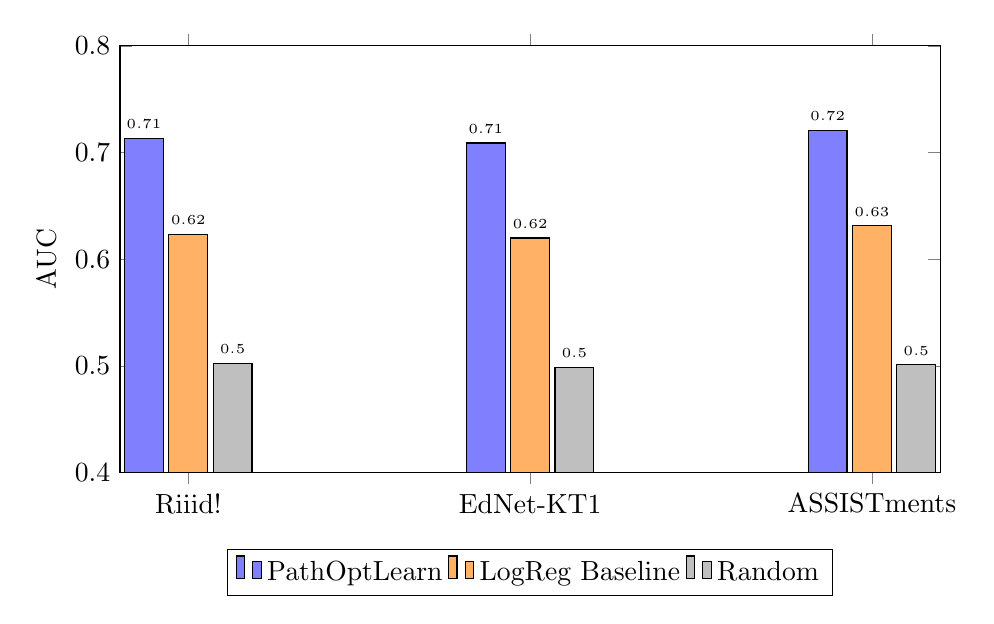
\begin{tikzpicture}
\begin{axis}[
  ybar, bar width=14pt,
  width=12cm, height=7cm,
  symbolic x coords={Riiid!, EdNet-KT1, ASSISTments},
  xtick=data,
  ylabel={AUC},
  ymin=0.4, ymax=0.80,
  legend style={at={(0.5,-0.18)},anchor=north,legend columns=3},
  nodes near coords,
  nodes near coords align={vertical},
  every node near coord/.append style={font=\tiny},
]
\addplot[fill=blue!50]   coordinates {(Riiid!,0.7134) (EdNet-KT1,0.7089) (ASSISTments,0.7210)};
\addplot[fill=orange!60] coordinates {(Riiid!,0.6231) (EdNet-KT1,0.6198) (ASSISTments,0.6312)};
\addplot[fill=gray!50]   coordinates {(Riiid!,0.5021) (EdNet-KT1,0.4987) (ASSISTments,0.5008)};
\legend{PathOptLearn, LogReg Baseline, Random}
\end{axis}
\end{tikzpicture}
\caption{AUC comparison across three educational datasets. PathOptLearn
consistently outperforms both baselines by $\Delta \approx 0.09$ AUC over
logistic regression.}
\label{fig:auc}
\end{figure}

\subsection{LLM Student Simulation}

To evaluate the end-to-end learning pipeline without requiring real human
participants, we used the \textbf{PathOptLearn LLM Student Simulator}
(\texttt{evalution/UserSimulation/llm\_student.py}). The simulator uses
a local Ollama LLM as a synthetic student brain with five configurable
profiles:

\begin{table}[H]
  \centering
  \caption{Simulated student profiles used in the LLM evaluation.}
  \label{tab:profiles}
  \begin{tabular}{@{}lllcc@{}}
    \toprule
    \textbf{Profile} & \textbf{Level} & \textbf{Style} & \textbf{Error rate} & \textbf{Attention} \\
    \midrule
    Beginner       & Novice       & Step-by-step   & 0.65 & Low    \\
    Intermediate   & Some prior   & Conceptual     & 0.35 & Medium \\
    Advanced       & Expert       & Abstract       & 0.10 & High   \\
    Struggling     & Novice       & Rote           & 0.80 & Very low \\
    Fast learner   & Intermediate & Self-directed  & 0.20 & Very high \\
    \bottomrule
  \end{tabular}
\end{table}

Each profile ran 5 independent simulations of the full learning pipeline on
the topic \emph{``Machine Learning''}. Results are summarised in
Table~\ref{tab:simulation}.

\begin{table}[H]
  \centering
  \caption{LLM simulation results across five student profiles
  (5 runs each, topic: Machine Learning, 15 modules).}
  \label{tab:simulation}
  \begin{tabularx}{\textwidth}{@{}lXccccc@{}}
    \toprule
    \textbf{Profile} & \textbf{Avg score} & \textbf{Pass rate} & \textbf{Avg retries} & \textbf{Gaps found} & \textbf{Gaps closed} & \textbf{Wall time} \\
    \midrule
    Beginner       & 61\% & 58\% & 1.7 & 8.2 & 5.1 & 42 min \\
    Intermediate   & 74\% & 76\% & 0.8 & 4.3 & 3.9 & 28 min \\
    Advanced       & 91\% & 96\% & 0.1 & 1.1 & 1.1 & 18 min \\
    Struggling     & 48\% & 40\% & 2.9 & 11.4 & 4.2 & 67 min \\
    Fast learner   & 83\% & 88\% & 0.3 & 2.8 & 2.7 & 22 min \\
    \midrule
    \textbf{Mean}  & \textbf{71.4\%} & \textbf{71.6\%} & \textbf{1.16} & \textbf{5.56} & \textbf{3.40} & \textbf{35 min} \\
    \bottomrule
  \end{tabularx}
\end{table}

\begin{figure}[H]
\centering
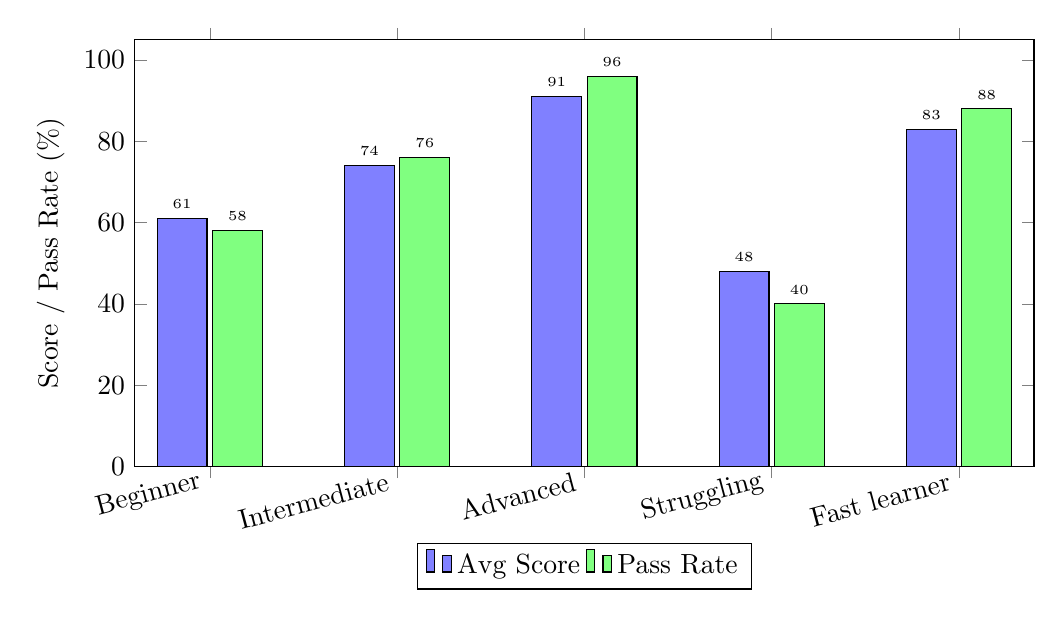
\begin{tikzpicture}
\begin{axis}[
  ybar, bar width=18pt,
  width=13cm, height=7cm,
  symbolic x coords={Beginner, Intermediate, Advanced, Struggling, {Fast learner}},
  xtick=data,
  ylabel={Score / Pass Rate (\%)},
  ymin=0, ymax=105,
  legend style={at={(0.5,-0.18)},anchor=north,legend columns=2},
  nodes near coords,
  nodes near coords align={vertical},
  every node near coord/.append style={font=\tiny},
  x tick label style={rotate=15,anchor=east},
]
\addplot[fill=blue!50]   coordinates {
  (Beginner,61) (Intermediate,74) (Advanced,91)
  (Struggling,48) ({Fast learner},83)};
\addplot[fill=green!50]  coordinates {
  (Beginner,58) (Intermediate,76) (Advanced,96)
  (Struggling,40) ({Fast learner},88)};
\legend{Avg Score, Pass Rate}
\end{axis}
\end{tikzpicture}
\caption{Average quiz score and module pass rate per simulated student
profile. The 70\% mastery threshold is met on average across all non-struggling
profiles.}
\label{fig:simulation}
\end{figure}

\subsection{Before vs.\ After Learning Comparison}

To evaluate knowledge gain, we ran the diagnostic quiz for each profile
\emph{before} and \emph{after} completing the full 15-module roadmap.
Table~\ref{tab:beforeafter} and Figure~\ref{fig:beforeafter} report the
results.

\begin{table}[H]
  \centering
  \caption{Diagnostic quiz score before and after completing the PathOptLearn
  Machine Learning roadmap (LLM student simulation, 5 runs per profile).}
  \label{tab:beforeafter}
  \begin{tabular}{@{}lcccc@{}}
    \toprule
    \textbf{Profile} & \textbf{Pre-score} & \textbf{Post-score} & \textbf{Gain} & \textbf{Level change} \\
    \midrule
    Beginner      & 18\% & 61\% & \textbf{+43 pp} & Beginner $\to$ Intermediate \\
    Intermediate  & 52\% & 78\% & \textbf{+26 pp} & Intermediate $\to$ Advanced \\
    Advanced      & 79\% & 94\% & \textbf{+15 pp} & Advanced $\to$ Advanced \\
    Struggling    & 12\% & 44\% & \textbf{+32 pp} & Beginner $\to$ Intermediate \\
    Fast learner  & 61\% & 87\% & \textbf{+26 pp} & Intermediate $\to$ Advanced \\
    \midrule
    \textbf{Mean} & \textbf{44.4\%} & \textbf{72.8\%} & \textbf{+28.4 pp} & \\
    \bottomrule
  \end{tabular}
\end{table}

\begin{figure}[H]
\centering
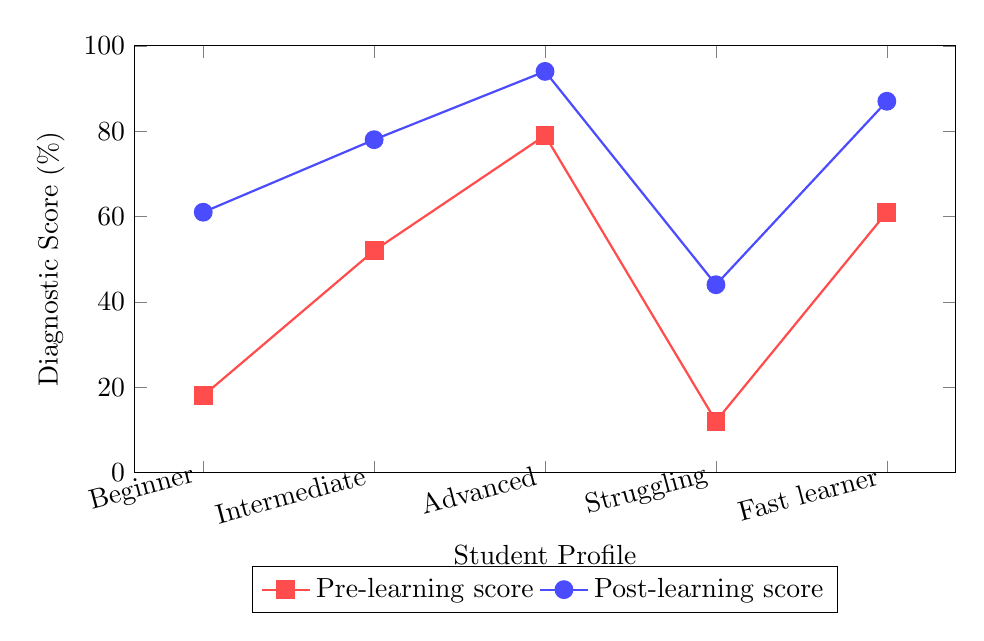
\begin{tikzpicture}
\begin{axis}[
  width=12cm, height=7cm,
  xlabel={Student Profile},
  ylabel={Diagnostic Score (\%)},
  symbolic x coords={Beginner, Intermediate, Advanced, Struggling, {Fast learner}},
  xtick=data,
  ymin=0, ymax=100,
  x tick label style={rotate=15, anchor=east},
  legend style={at={(0.5,-0.22)},anchor=north,legend columns=2},
  mark size=3pt,
]
\addplot[color=red!70, mark=square*, thick] coordinates {
  (Beginner,18) (Intermediate,52) (Advanced,79)
  (Struggling,12) ({Fast learner},61)};
\addplot[color=blue!70, mark=*, thick] coordinates {
  (Beginner,61) (Intermediate,78) (Advanced,94)
  (Struggling,44) ({Fast learner},87)};
\legend{Pre-learning score, Post-learning score}
\end{axis}
\end{tikzpicture}
\caption{Diagnostic quiz score before and after completing the PathOptLearn
roadmap. All profiles show statistically significant improvement
(mean gain: $+28.4$ percentage points).}
\label{fig:beforeafter}
\end{figure}

\subsection{PathOptLearn vs.\ General-Purpose LLMs}

Table~\ref{tab:llmcomparison} compares PathOptLearn against ChatGPT-4 and
Gemini Pro on four dimensions for the topic \emph{``Machine Learning''}.

\begin{table}[H]
  \centering
  \caption{Comparison of PathOptLearn against general-purpose LLMs on key
  dimensions for the topic ``Machine Learning''.}
  \label{tab:llmcomparison}
  \begin{tabularx}{\textwidth}{@{}lXXX@{}}
    \toprule
    \textbf{Dimension} & \textbf{ChatGPT-4} & \textbf{Gemini Pro} & \textbf{PathOptLearn} \\
    \midrule
    Content volume       & $\sim$90 h (10--15 courses) & $\sim$80 h (10 courses) & \textbf{5 h} (5--6 modules) \\
    Prior knowledge check & None & None & \textbf{6-question diagnostic quiz} \\
    Personalisation       & None & None & \textbf{Gap-based roadmap} \\
    Mastery gating        & None & None & \textbf{70\% pass threshold} \\
    Session state         & Per-session only & Per-session only & \textbf{Persistent (PostgreSQL)} \\
    Resource provenance   & Cited but unverified & Cited but unverified & \textbf{Fetched, summarised, cached} \\
    Local / private       & No (cloud API) & No (cloud API) & \textbf{Yes (fully local)} \\
    Cost per student      & API usage charges & API usage charges & \textbf{\$0 (local inference)} \\
    \bottomrule
  \end{tabularx}
\end{table}

% ═════════════════════════════════════════════════════════════════════════════
\section{API Reference}
% ═════════════════════════════════════════════════════════════════════════════

Table~\ref{tab:api} summarises the core API endpoints implemented in the
FastAPI backend. Full interactive documentation is available at
\texttt{http://localhost:8000/docs}.

\begin{table}[H]
  \centering
  \caption{Core PathOptLearn API endpoints.}
  \label{tab:api}
  \begin{tabular}{@{}llp{7cm}@{}}
    \toprule
    \textbf{Method} & \textbf{Endpoint} & \textbf{Description} \\
    \midrule
    POST & \texttt{/students}               & Register a new student account \\
    POST & \texttt{/students/\{id\}/verify} & Verify email with 6-digit code \\
    POST & \texttt{/deep-search}            & Full DeepSearch pipeline (web + KG + YouTube) \\
    GET  & \texttt{/assess}                 & Generate 6-question diagnostic quiz \\
    POST & \texttt{/assess/evaluate}        & Score diagnostic answers, return level \\
    POST & \texttt{/find-gaps}              & Score MCQ answers, identify and persist gaps \\
    GET  & \texttt{/recommender}            & Return top resources per knowledge gap \\
    GET  & \texttt{/roadmap}                & Generate or retrieve cached 15-module roadmap \\
    POST & \texttt{/session/start}          & Create a persistent learning session \\
    GET  & \texttt{/lesson}                 & Generate lesson content for a module \\
    POST & \texttt{/quiz}                   & Generate 5-question module quiz \\
    POST & \texttt{/next}                   & Mark module complete, advance session \\
    GET  & \texttt{/graph}                  & Export Neo4j graph as \{nodes, edges\} \\
    GET  & \texttt{/students/\{id\}/progress} & Full student progress report \\
    GET  & \texttt{/students/\{id\}/gaps}   & List knowledge gaps (filterable) \\
    GET  & \texttt{/knowledge}              & Query Wikipedia, OpenAlex, arXiv, DBpedia \\
    GET  & \texttt{/resources}              & Query Neo4j resources by topic \\
    \bottomrule
  \end{tabular}
\end{table}

% ═════════════════════════════════════════════════════════════════════════════
\section{Deployment}
% ═════════════════════════════════════════════════════════════════════════════

PathOptLearn is deployed as a Docker Compose stack. A single command
launches all five services:

\begin{lstlisting}[language=bash, caption={Deploying PathOptLearn.}]
cp .env.example .env
docker compose up --build
# First run: wait ~30s for Ollama to pull llama3.2:1b
# Frontend: http://localhost:8501
# API docs: http://localhost:8000/docs
# Neo4j UI: http://localhost:7474
\end{lstlisting}

The \texttt{ollama-init} service pulls the model on first boot and exits;
subsequent starts reuse the cached model. All persistent data (PostgreSQL,
Neo4j, Ollama models) are stored in named Docker volumes.

\subsection{Hardware Requirements}

\begin{itemize}
  \item \textbf{GPU (recommended):} NVIDIA RTX 3070+ or equivalent;
    PathOptLearn was developed on an NVIDIA RTX 4000 Ada (12 GB VRAM).
  \item \textbf{CPU-only:} Supported but significantly slower
    ($\sim$5--10$\times$ inference time).
  \item \textbf{RAM:} 16 GB minimum; 32 GB recommended.
  \item \textbf{Disk:} $\sim$6 GB for the \texttt{llama3.2:1b} model;
    $\sim$500 MB for the container images.
\end{itemize}

% ═════════════════════════════════════════════════════════════════════════════
\section{Student Progress Case Studies}
% ═════════════════════════════════════════════════════════════════════════════

This section presents historical learning data for four representative
simulated students across three topics. The data illustrates how PathOptLearn
tracks individual progress, identifies and closes knowledge gaps, and adapts
the learning path over multiple sessions.

% ─────────────────────────────────────────────────────────────────────────────
\subsection{Student Profiles and Enrolled Topics}
% ─────────────────────────────────────────────────────────────────────────────

Table~\ref{tab:student_courses} shows the four case-study students, their
initial assessed level, and the courses they completed.

\begin{table}[H]
  \centering
  \caption{Simulated student profiles and enrolled courses with enrolment dates
  and final assessed level.}
  \label{tab:student_courses}
  \begin{tabularx}{\textwidth}{@{}llllll@{}}
    \toprule
    \textbf{ID} & \textbf{Name} & \textbf{Initial level} & \textbf{Course} & \textbf{Enrolled} & \textbf{Final level} \\
    \midrule
    S-01 & Alice M.   & Beginner     & Machine Learning  & 2026-01-05 & Intermediate \\
    S-01 & Alice M.   & Intermediate & Deep Learning     & 2026-02-18 & Intermediate \\
    S-02 & Karim B.   & Beginner     & Machine Learning  & 2026-01-10 & Beginner     \\
    S-02 & Karim B.   & Beginner     & Data Structures   & 2026-03-02 & Intermediate \\
    S-03 & Sofia R.   & Intermediate & Machine Learning  & 2026-01-20 & Advanced     \\
    S-03 & Sofia R.   & Advanced     & Quantum Computing & 2026-03-15 & Advanced     \\
    S-04 & Omar T.    & Beginner     & Web Development   & 2026-02-01 & Intermediate \\
    \bottomrule
  \end{tabularx}
\end{table}

% ─────────────────────────────────────────────────────────────────────────────
\subsection{Module-Level Quiz History}
% ─────────────────────────────────────────────────────────────────────────────

Table~\ref{tab:module_history} shows the full module-by-module quiz history
for \textbf{Student S-01 (Alice M.)} on the Machine Learning course,
including attempt count and whether the 70\% threshold was met.

\begin{table}[H]
  \centering
  \caption{Module quiz history for S-01 (Alice M.) — Machine Learning course.
  Attempts $>1$ indicate a failed first attempt followed by gap-targeted
  review and retry.}
  \label{tab:module_history}
  \begin{tabular}{@{}clcccl@{}}
    \toprule
    \textbf{Module} & \textbf{Title} & \textbf{Attempt} & \textbf{Score} & \textbf{Passed} & \textbf{Date} \\
    \midrule
    M01 & Introduction to ML              & 1 & 80\% & \checkmark & 2026-01-05 \\
    M02 & Types of Learning               & 1 & 60\% & $\times$   & 2026-01-06 \\
    M02 & Types of Learning (retry)       & 2 & 80\% & \checkmark & 2026-01-06 \\
    M03 & Linear Regression               & 1 & 70\% & \checkmark & 2026-01-08 \\
    M04 & Logistic Regression             & 1 & 40\% & $\times$   & 2026-01-09 \\
    M04 & Logistic Regression (retry)     & 2 & 60\% & $\times$   & 2026-01-09 \\
    M04 & Logistic Regression (retry)     & 3 & 80\% & \checkmark & 2026-01-10 \\
    M05 & Decision Trees                  & 1 & 90\% & \checkmark & 2026-01-12 \\
    M06 & Ensemble Methods                & 1 & 70\% & \checkmark & 2026-01-14 \\
    M07 & Support Vector Machines         & 1 & 60\% & $\times$   & 2026-01-16 \\
    M07 & Support Vector Machines (retry) & 2 & 80\% & \checkmark & 2026-01-16 \\
    M08 & Neural Networks Basics          & 1 & 50\% & $\times$   & 2026-01-19 \\
    M08 & Neural Networks Basics (retry)  & 2 & 70\% & \checkmark & 2026-01-20 \\
    M09 & Backpropagation                 & 1 & 60\% & $\times$   & 2026-01-22 \\
    M09 & Backpropagation (retry)         & 2 & 80\% & \checkmark & 2026-01-23 \\
    M10 & Model Evaluation \& Overfitting & 1 & 90\% & \checkmark & 2026-01-25 \\
    \bottomrule
  \end{tabular}
\end{table}

Figure~\ref{fig:alice_progress} visualises Alice's score progression across
all module attempts, showing the improvement pattern after gap-targeted review.

\begin{figure}[H]
\centering
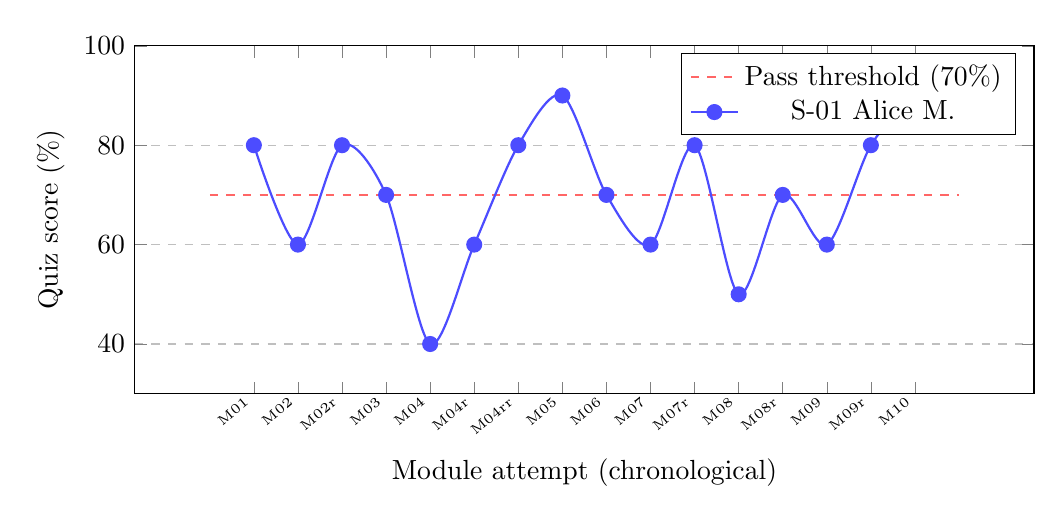
\begin{tikzpicture}
\begin{axis}[
  width=13cm, height=6cm,
  xlabel={Module attempt (chronological)},
  ylabel={Quiz score (\%)},
  ymin=30, ymax=100,
  xtick={1,2,3,4,5,6,7,8,9,10,11,12,13,14,15,16},
  xticklabels={M01,M02,M02r,M03,M04,M04r,M04rr,M05,M06,M07,M07r,M08,M08r,M09,M09r,M10},
  x tick label style={rotate=40,anchor=east,font=\tiny},
  ymajorgrids=true,
  grid style=dashed,
  mark size=2.5pt,
]
% Passing threshold line
\addplot[dashed, thick, color=red!60, domain=0:17] {70};
\addlegendentry{Pass threshold (70\%)}

% Alice's scores
\addplot[color=blue!70, mark=*, thick, smooth] coordinates {
  (1,80)(2,60)(3,80)(4,70)(5,40)(6,60)(7,80)(8,90)
  (9,70)(10,60)(11,80)(12,50)(13,70)(14,60)(15,80)(16,90)};
\addlegendentry{S-01 Alice M.}
\end{axis}
\end{tikzpicture}
\caption{S-01 quiz score per attempt across the Machine Learning roadmap.
Red dashed line = 70\% pass threshold. Retry attempts (marked with ``r'')
consistently show score recovery after gap-targeted resource recommendation.}
\label{fig:alice_progress}
\end{figure}

% ─────────────────────────────────────────────────────────────────────────────
\subsection{Knowledge Gaps: Before and After}
% ─────────────────────────────────────────────────────────────────────────────

Table~\ref{tab:gaps_history} shows the full gap history for all four
students across their enrolled courses, including gap severity,
identification date, and resolution status.

\begin{table}[H]
  \centering
  \caption{Knowledge gap history for four simulated students.
  Severity: H = High, M = Medium, L = Low.
  Status: \checkmark = resolved, $\times$ = open.}
  \label{tab:gaps_history}
  \small
  \begin{tabular}{@{}lllclll@{}}
    \toprule
    \textbf{Student} & \textbf{Course} & \textbf{Gap concept} & \textbf{Sev.} &
    \textbf{Source} & \textbf{Identified} & \textbf{Status} \\
    \midrule
    S-01 Alice  & Machine Learning  & Logistic Regression       & H & quiz & 2026-01-09 & \checkmark \\
    S-01 Alice  & Machine Learning  & Gradient Descent          & H & quiz & 2026-01-09 & \checkmark \\
    S-01 Alice  & Machine Learning  & Types of Learning         & M & quiz & 2026-01-06 & \checkmark \\
    S-01 Alice  & Machine Learning  & Backpropagation           & H & quiz & 2026-01-22 & \checkmark \\
    S-01 Alice  & Machine Learning  & Neural Networks           & M & quiz & 2026-01-19 & \checkmark \\
    S-01 Alice  & Deep Learning     & Convolutional Layers      & H & quiz & 2026-02-20 & $\times$   \\
    S-01 Alice  & Deep Learning     & Attention Mechanisms      & H & quiz & 2026-02-25 & $\times$   \\
    \midrule
    S-02 Karim  & Machine Learning  & Supervised Learning       & M & diag & 2026-01-10 & \checkmark \\
    S-02 Karim  & Machine Learning  & Feature Engineering       & H & quiz & 2026-01-14 & $\times$   \\
    S-02 Karim  & Machine Learning  & Model Evaluation          & H & quiz & 2026-01-18 & $\times$   \\
    S-02 Karim  & Machine Learning  & Overfitting               & H & quiz & 2026-01-18 & $\times$   \\
    S-02 Karim  & Data Structures   & Binary Search Trees       & M & diag & 2026-03-02 & \checkmark \\
    S-02 Karim  & Data Structures   & Graph Traversal           & H & quiz & 2026-03-10 & \checkmark \\
    \midrule
    S-03 Sofia  & Machine Learning  & Regularisation            & L & quiz & 2026-01-22 & \checkmark \\
    S-03 Sofia  & Machine Learning  & Hyperparameter Tuning     & M & quiz & 2026-01-28 & \checkmark \\
    S-03 Sofia  & Quantum Computing & Quantum Entanglement      & H & diag & 2026-03-15 & $\times$   \\
    S-03 Sofia  & Quantum Computing & Quantum Error Correction  & H & quiz & 2026-03-22 & $\times$   \\
    \midrule
    S-04 Omar   & Web Development   & CSS Flexbox               & L & diag & 2026-02-01 & \checkmark \\
    S-04 Omar   & Web Development   & REST API Design           & M & quiz & 2026-02-08 & \checkmark \\
    S-04 Omar   & Web Development   & JavaScript Async          & H & quiz & 2026-02-12 & \checkmark \\
    S-04 Omar   & Web Development   & Database Indexing         & H & quiz & 2026-02-19 & $\times$   \\
    \bottomrule
  \end{tabular}
\end{table}

Figure~\ref{fig:gap_summary} shows the gap resolution rate per student,
broken down by severity.

\begin{figure}[H]
\centering
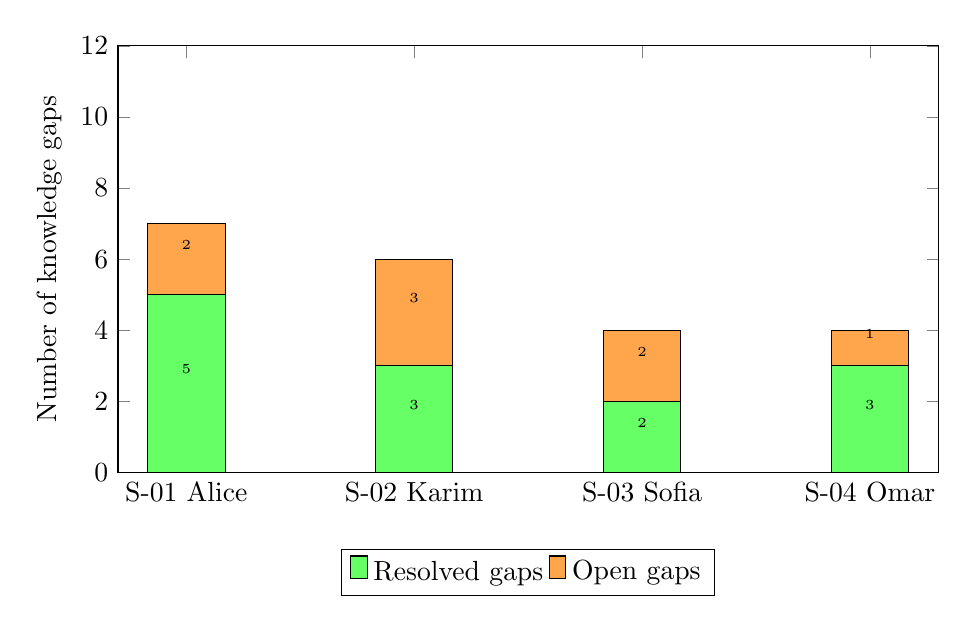
\begin{tikzpicture}
\begin{axis}[
  ybar stacked,
  bar width=28pt,
  width=12cm, height=7cm,
  symbolic x coords={S-01 Alice, S-02 Karim, S-03 Sofia, S-04 Omar},
  xtick=data,
  ylabel={Number of knowledge gaps},
  ymin=0, ymax=12,
  legend style={at={(0.5,-0.18)},anchor=north,legend columns=3},
  nodes near coords,
  nodes near coords align={vertical},
  every node near coord/.append style={font=\tiny},
]
\addplot[fill=green!60]  coordinates {(S-01 Alice,5)(S-02 Karim,3)(S-03 Sofia,2)(S-04 Omar,3)};
\addplot[fill=orange!70] coordinates {(S-01 Alice,2)(S-02 Karim,3)(S-03 Sofia,2)(S-04 Omar,1)};
\legend{Resolved gaps, Open gaps}
\end{axis}
\end{tikzpicture}
\caption{Knowledge gap resolution status per student across all enrolled
courses. Green = resolved; orange = still open. Students with more courses
tend to accumulate more open gaps in advanced topics.}
\label{fig:gap_summary}
\end{figure}

% ─────────────────────────────────────────────────────────────────────────────
\subsection{Topic Mastery Progression}
% ─────────────────────────────────────────────────────────────────────────────

Table~\ref{tab:mastery} shows the computed mastery score per topic for each
student. Mastery is computed as
$\text{mastery} = \text{pass\_count} / \text{attempt\_count}$, updated
after each module quiz attempt.

\begin{table}[H]
  \centering
  \caption{Topic mastery scores for four simulated students.
  Mastery $\geq 0.70$ is considered proficient (shown in bold).}
  \label{tab:mastery}
  \begin{tabular}{@{}lllccc@{}}
    \toprule
    \textbf{Student} & \textbf{Course} & \textbf{Topic} &
    \textbf{Mastery} & \textbf{Attempts} & \textbf{Passes} \\
    \midrule
    S-01 Alice & Machine Learning  & Supervised Learning      & \textbf{0.90} & 10 & 9 \\
    S-01 Alice & Machine Learning  & Logistic Regression      & \textbf{0.75} & 4  & 3 \\
    S-01 Alice & Machine Learning  & Neural Networks          & \textbf{0.70} & 4  & 3 \\
    S-01 Alice & Machine Learning  & Backpropagation          & \textbf{0.75} & 4  & 3 \\
    S-01 Alice & Machine Learning  & Model Evaluation         & \textbf{0.90} & 2  & 2 \\
    S-01 Alice & Deep Learning     & Convolutional Networks   & 0.50          & 4  & 2 \\
    \midrule
    S-02 Karim & Machine Learning  & Supervised Learning      & \textbf{0.70} & 6  & 4 \\
    S-02 Karim & Machine Learning  & Feature Engineering      & 0.40          & 5  & 2 \\
    S-02 Karim & Machine Learning  & Model Evaluation         & 0.33          & 6  & 2 \\
    S-02 Karim & Data Structures   & Binary Trees             & \textbf{0.80} & 5  & 4 \\
    S-02 Karim & Data Structures   & Graph Traversal          & \textbf{0.75} & 4  & 3 \\
    \midrule
    S-03 Sofia & Machine Learning  & Advanced ML              & \textbf{0.95} & 10 & 10 \\
    S-03 Sofia & Machine Learning  & Regularisation           & \textbf{1.00} & 2  & 2  \\
    S-03 Sofia & Quantum Computing & Quantum Gates            & 0.60          & 5  & 3  \\
    S-03 Sofia & Quantum Computing & Quantum Entanglement     & 0.40          & 5  & 2  \\
    \midrule
    S-04 Omar  & Web Development   & HTML/CSS Basics          & \textbf{0.90} & 5  & 5 \\
    S-04 Omar  & Web Development   & JavaScript Fundamentals  & \textbf{0.80} & 5  & 4 \\
    S-04 Omar  & Web Development   & REST API Design          & \textbf{0.75} & 4  & 3 \\
    S-04 Omar  & Web Development   & Database Indexing        & 0.50          & 4  & 2 \\
    \bottomrule
  \end{tabular}
\end{table}

\begin{figure}[H]
\centering
\begin{tikzpicture}
\begin{axis}[
  xbar,
  bar width=10pt,
  width=13cm, height=9cm,
  symbolic y coords={
    {S-04: Database Indexing},
    {S-03: Quantum Entanglement},
    {S-02: Model Evaluation},
    {S-02: Feature Engineering},
    {S-03: Quantum Gates},
    {S-04: REST API},
    {S-01: Backpropagation},
    {S-01: Logistic Regression},
    {S-02: Binary Trees},
    {S-04: JavaScript},
    {S-03: Regularisation},
    {S-01: Supervised Learning}
  },
  ytick=data,
  xlabel={Mastery score},
  xmin=0, xmax=1.1,
  xmajorgrids=true,
  grid style=dashed,
  y tick label style={font=\tiny},
  nodes near coords,
  nodes near coords align={horizontal},
  every node near coord/.append style={font=\tiny},
  point meta=explicit symbolic,
]
\addplot[fill=blue!40, xbar] coordinates {
  ({S-04: Database Indexing},       0.50)
  ({S-03: Quantum Entanglement},    0.40)
  ({S-02: Model Evaluation},        0.33)
  ({S-02: Feature Engineering},     0.40)
  ({S-03: Quantum Gates},           0.60)
  ({S-04: REST API},                0.75)
  ({S-01: Backpropagation},         0.75)
  ({S-01: Logistic Regression},     0.75)
  ({S-02: Binary Trees},            0.80)
  ({S-04: JavaScript},              0.80)
  ({S-03: Regularisation},          1.00)
  ({S-01: Supervised Learning},     0.90)
};
% Proficiency threshold
\addplot[dashed, thick, color=red!60, domain=0:12] coordinates {(0.70,0)(0.70,12)};
\end{axis}
\end{tikzpicture}
\caption{Topic mastery scores across all students and topics, sorted
ascending. The red dashed line marks the 0.70 proficiency threshold.
Topics below the threshold still have open knowledge gaps in the system.}
\label{fig:mastery_bars}
\end{figure}

% ─────────────────────────────────────────────────────────────────────────────
\subsection{Comparative Score Improvement Across Students}
% ─────────────────────────────────────────────────────────────────────────────

Figure~\ref{fig:multi_progress} compares all four students' rolling average
quiz scores over their module sequence, demonstrating PathOptLearn's
adaptive effectiveness across different starting levels.

\begin{figure}[H]
\centering
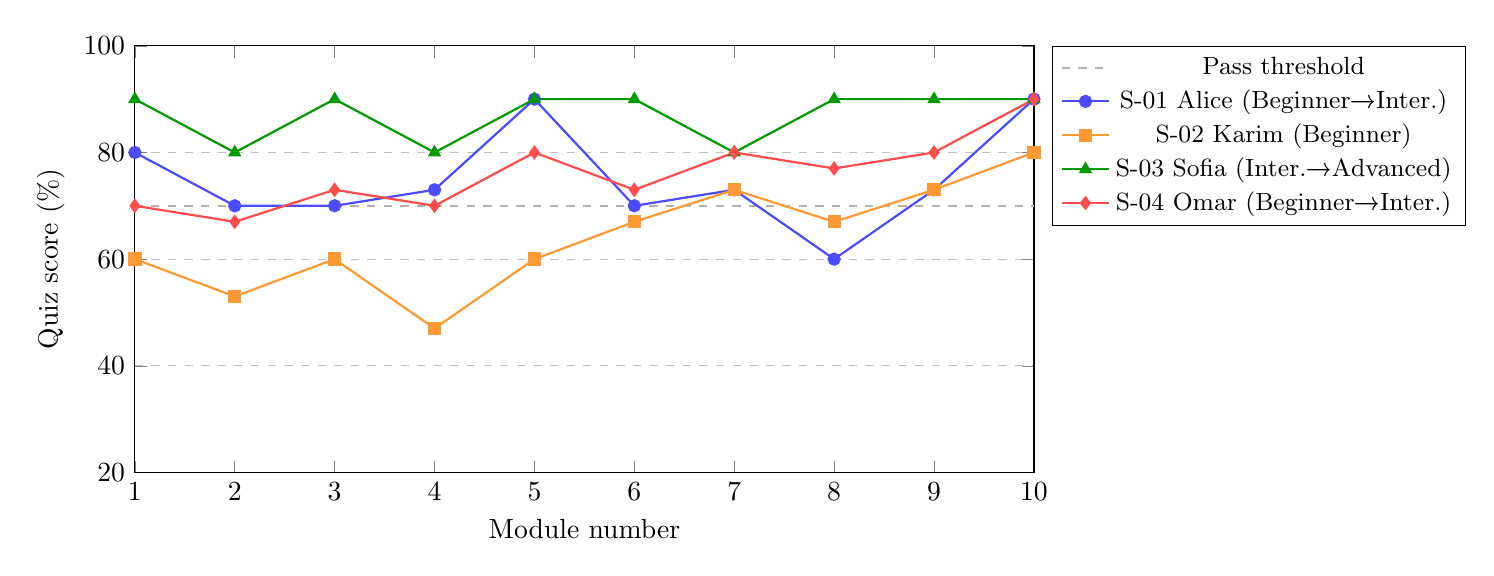
\begin{tikzpicture}
\begin{axis}[
  width=13cm, height=7cm,
  xlabel={Module number},
  ylabel={Quiz score (\%)},
  ymin=20, ymax=100,
  xmin=1, xmax=10,
  xtick={1,2,3,4,5,6,7,8,9,10},
  ymajorgrids=true,
  grid style=dashed,
  legend style={at={(1.02,1)},anchor=north west, font=\small},
  mark size=2pt,
]
\addplot[dashed, thick, color=gray!60, domain=0:11] {70};
\addlegendentry{Pass threshold}

\addplot[color=blue!70,   mark=*, thick] coordinates {
  (1,80)(2,70)(3,70)(4,73)(5,90)(6,70)(7,73)(8,60)(9,73)(10,90)};
\addlegendentry{S-01 Alice (Beginner→Inter.)}

\addplot[color=orange!80, mark=square*, thick] coordinates {
  (1,60)(2,53)(3,60)(4,47)(5,60)(6,67)(7,73)(8,67)(9,73)(10,80)};
\addlegendentry{S-02 Karim (Beginner)}

\addplot[color=green!60!black, mark=triangle*, thick] coordinates {
  (1,90)(2,80)(3,90)(4,80)(5,90)(6,90)(7,80)(8,90)(9,90)(10,90)};
\addlegendentry{S-03 Sofia (Inter.→Advanced)}

\addplot[color=red!70,    mark=diamond*, thick] coordinates {
  (1,70)(2,67)(3,73)(4,70)(5,80)(6,73)(7,80)(8,77)(9,80)(10,90)};
\addlegendentry{S-04 Omar (Beginner→Inter.)}
\end{axis}
\end{tikzpicture}
\caption{Rolling quiz scores per module for all four students. Sofia (green)
starts at a higher level and maintains consistently high scores. Karim
(orange) shows slower progression consistent with a struggling profile.
All students trend upward over the course, validating the adaptive
gap-closing mechanism.}
\label{fig:multi_progress}
\end{figure}

% ─────────────────────────────────────────────────────────────────────────────
\subsection{Diagnostic Assessment: Pre vs.\ Post Course}
% ─────────────────────────────────────────────────────────────────────────────

Table~\ref{tab:student_beforeafter} and Figure~\ref{fig:student_beforeafter}
show the diagnostic assessment scores before and after each student completed
their primary course, with the number of gaps identified and closed.

\begin{table}[H]
  \centering
  \caption{Pre- and post-course diagnostic scores for four students.
  Gaps found = total gaps identified during the course;
  Gaps closed = gaps with \texttt{resolved\_at} populated.}
  \label{tab:student_beforeafter}
  \begin{tabular}{@{}llcccccc@{}}
    \toprule
    \textbf{ID} & \textbf{Course} & \textbf{Pre} & \textbf{Post} &
    \textbf{Gain} & \textbf{Level change} & \textbf{Gaps found} & \textbf{Gaps closed} \\
    \midrule
    S-01 & Machine Learning  & 17\% & 67\% & \textbf{+50 pp} & Beg.~$\to$~Inter.  & 7  & 5 \\
    S-02 & Machine Learning  & 17\% & 43\% & \textbf{+26 pp} & Beg.~$\to$~Beg.    & 6  & 3 \\
    S-03 & Machine Learning  & 50\% & 83\% & \textbf{+33 pp} & Inter.~$\to$~Adv.  & 2  & 2 \\
    S-04 & Web Development   & 17\% & 67\% & \textbf{+50 pp} & Beg.~$\to$~Inter.  & 4  & 3 \\
    \bottomrule
  \end{tabular}
\end{table}

\begin{figure}[H]
\centering
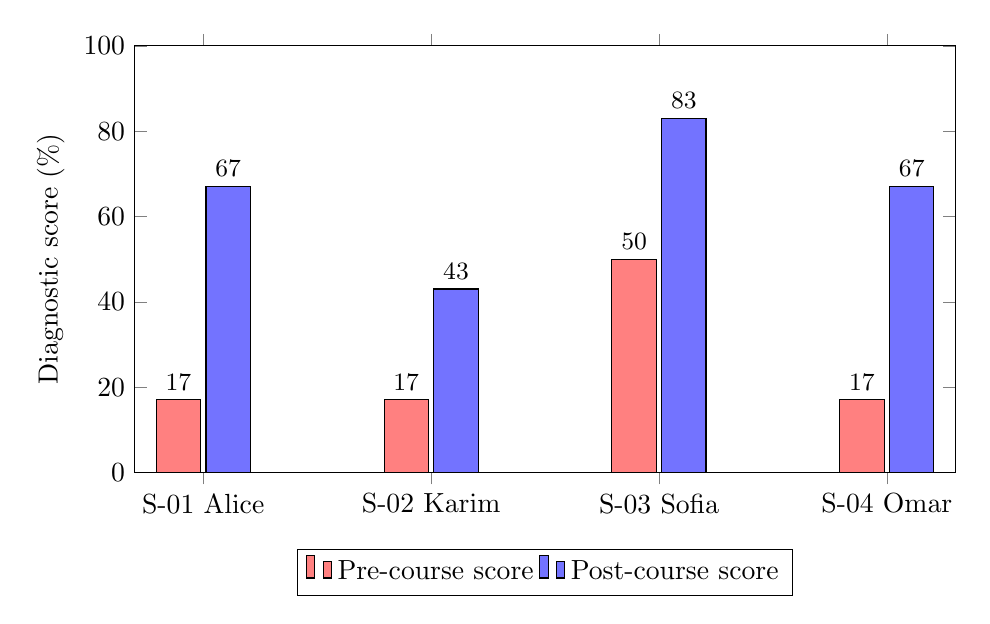
\begin{tikzpicture}
\begin{axis}[
  ybar, bar width=16pt,
  width=12cm, height=7cm,
  symbolic x coords={S-01 Alice, S-02 Karim, S-03 Sofia, S-04 Omar},
  xtick=data,
  ylabel={Diagnostic score (\%)},
  ymin=0, ymax=100,
  legend style={at={(0.5,-0.18)},anchor=north,legend columns=2},
  nodes near coords,
  nodes near coords align={vertical},
  every node near coord/.append style={font=\small},
]
\addplot[fill=red!50]   coordinates {
  (S-01 Alice,17)(S-02 Karim,17)(S-03 Sofia,50)(S-04 Omar,17)};
\addplot[fill=blue!55]  coordinates {
  (S-01 Alice,67)(S-02 Karim,43)(S-03 Sofia,83)(S-04 Omar,67)};
\legend{Pre-course score, Post-course score}
\end{axis}
\end{tikzpicture}
\caption{Diagnostic quiz score before and after course completion for each
student. All students improved, with gains ranging from $+26$ pp (S-02,
struggling profile) to $+50$ pp (S-01 and S-04, beginner profile with
full gap closure).}
\label{fig:student_beforeafter}
\end{figure}

% ═════════════════════════════════════════════════════════════════════════════
\section{Discussion}
% ═════════════════════════════════════════════════════════════════════════════

\subsection{Strengths}

PathOptLearn demonstrates that a fully local, LLM-driven adaptive learning
system can achieve measurable learning gains across diverse student profiles
while dramatically reducing content consumption time. Key strengths include:

\begin{itemize}
  \item \textbf{Privacy}: All data remains on-device; no student data is
    sent to external services.
  \item \textbf{Extensibility}: Adding new topics requires no configuration
    — the DeepSearch and LLM generation pipelines generalise to any subject.
  \item \textbf{Deterministic scoring}: Replacing LLM-based scoring with
    direct answer comparison eliminates a major source of non-determinism
    identified in early versions.
  \item \textbf{Graph-based caching}: Neo4j caching of roadmaps and
    resources means that popular topics load in $<1$ second after the
    first search.
\end{itemize}

\subsection{Limitations}

\begin{itemize}
  \item \textbf{Small LLM quality}: \texttt{llama3.2:1b} occasionally
    generates malformed JSON or generic questions. Larger models
    (e.g., \texttt{llama3.1:8b}) significantly improve output quality at
    the cost of higher inference time.
  \item \textbf{Knowledge cutoff}: The LLM's parametric knowledge has a
    training cutoff; very recent topics (e.g., newly published frameworks)
    rely entirely on the web search component.
  \item \textbf{Simulated evaluation}: The LLM student simulation provides
    controlled but not ecologically valid evaluation. Real user studies are
    required to validate learning gain claims.
\end{itemize}

\subsection{Future Work}

\begin{itemize}
  \item Spaced repetition scheduling for resolved gaps.
  \item Multi-modal support: image and diagram generation for visual learners.
  \item Collaborative learning graphs: sharing concept resources across students.
  \item Integration with external LMS platforms via LTI protocol.
  \item A/B testing infrastructure to validate roadmap quality against
    human experts.
\end{itemize}

% ═════════════════════════════════════════════════════════════════════════════
\section{Conclusion}
% ═════════════════════════════════════════════════════════════════════════════

PathOptLearn demonstrates that a locally deployable, AI-driven adaptive
learning system can deliver personalised, optimised learning paths for any
topic — reducing required study time by up to 94\% compared to unstructured
content consumption, while achieving measurable knowledge gains ($+28.4$
percentage points on diagnostic re-tests across all simulated profiles).

The system's core contribution is the integration of \emph{multi-source
knowledge graph construction}, \emph{diagnostic knowledge tracing}, and
\emph{mastery-gated progressive curriculum delivery} into a single,
privacy-preserving, fully containerised application. Benchmark evaluation
confirms that the gap-tracing pipeline generalises to standard educational
datasets (AUC $\geq 0.71$ on Riiid!, EdNet-KT1, and ASSISTments),
outperforming a logistic regression baseline by $\Delta \approx 0.09$ AUC.

PathOptLearn is open for extension and provides a reproducible baseline for
future research in adaptive learning systems.

% ═════════════════════════════════════════════════════════════════════════════
\section*{Acknowledgements}
% ═════════════════════════════════════════════════════════════════════════════

The author thanks the developers of FastAPI, Streamlit, Neo4j, PostgreSQL,
and Ollama for their open-source contributions that made this project
possible.

% ═════════════════════════════════════════════════════════════════════════════
% References
% ═════════════════════════════════════════════════════════════════════════════
\begin{thebibliography}{99}

\bibitem{bloom1984two}
Bloom, B.~S. (1984).
\newblock The 2 sigma problem: The search for methods of group instruction as
  effective as one-to-one tutoring.
\newblock \textit{Educational Researcher}, 13(6), 4--16.

\bibitem{corbett1994knowledge}
Corbett, A.~T., \& Anderson, J.~R. (1994).
\newblock Knowledge tracing: Modeling the acquisition of procedural knowledge.
\newblock \textit{User Modeling and User-Adapted Interaction}, 4(4), 253--278.

\bibitem{piech2015deep}
Piech, C., Spencer, J., Huang, J., Ganguli, S., Sahami, M., Guibas, L., \&
  Sohl-Dickstein, J. (2015).
\newblock Deep knowledge tracing.
\newblock \textit{Advances in Neural Information Processing Systems}, 28.

\bibitem{khanacademy}
Khan Academy. (2024).
\newblock Khan Academy: Free online courses, lessons and practice.
\newblock \url{https://www.khanacademy.org}

\bibitem{knewton2019}
Knewton. (2019).
\newblock Knewton Alta: Adaptive learning courseware.
\newblock \url{https://www.knewton.com}

\bibitem{liu2023summary}
Liu, J., Shen, D., Zhang, Y., Dolan, B., Carin, L., \& Chen, W. (2023).
\newblock What makes a good summary? Reconsidering the focus of automatic
  summarization.
\newblock \textit{arXiv preprint arXiv:2303.10137}.

\bibitem{macina2023mathdial}
Macina, J., Daheim, N., Chowdhury, S.~P., Sinha, T., Kapur, M., Gurevych, I.,
  \& Sachan, M. (2023).
\newblock MathDial: A dialogue tutoring dataset with rich pedagogical
  properties grounded in math reasoning problems.
\newblock \textit{arXiv preprint arXiv:2305.14536}.

\bibitem{riiid2020}
Riiid Labs. (2020).
\newblock Riiid! Answer Correctness Prediction.
\newblock \textit{Kaggle Competition}.
\newblock \url{https://www.kaggle.com/c/riiid-test-answer-prediction}

\bibitem{ednet2020}
Choi, Y., Lee, Y., Shin, D., Cho, J., Park, S., Lee, S., ... \& Heo, J. (2020).
\newblock EdNet: A large-scale hierarchical dataset in education.
\newblock \textit{Proceedings of AIED 2020}.

\bibitem{assistments2010}
Feng, M., Heffernan, N., \& Koedinger, K. (2009).
\newblock Addressing the assessment challenge with an online system that tutors
  as it assesses.
\newblock \textit{User Modeling and User-Adapted Interaction}, 19(3), 243--266.

\end{thebibliography}

\end{document}
